Originally, it was intended to display the networks in 2D, with a 3D representation being considered a nice to have feature. During testing we found that a 2D representation does not provide a clear view of the network. Even for relatively small networks (\~200 nodes) the 2D representation was very confusing. For this reason, the 2D representation was scrapped and only the 3D one was implemented. In 3D, even networks with thousands of nodes provide a clear view of the different groups and nodes.
\newline

The Python package plotly \cite{plotly} is used to display the networks in 3D. \texttt{plotly.graph\_objs} provides the \texttt{Scatter3d} function, which is used to draw both the nodes and edges. For the nodes the function takes in three lists of coordinates, one for each axis x, y and z. For the edges it also requires these three lists, but here the first coordinate is the start point for an edge, the second the end point, followed by a None entry and then the next edge coordinates. Currently, the only information that is generated for graphs is the number of nodes in each group and lists of which node ids must be connected with edges. This information must be translated into coordinates for plotly to be able to display the network.

\section{Displaying the nodes}
\label{sub:displayNodes}
All nodes belonging to the same group should be arranged in a sphere. Each sphere thus represents one group and the spheres must have enough space between them so that the groups can be easily distinguished, as shown in Figure \ref{fig:groups}.

\begin{figure}
    \centering
    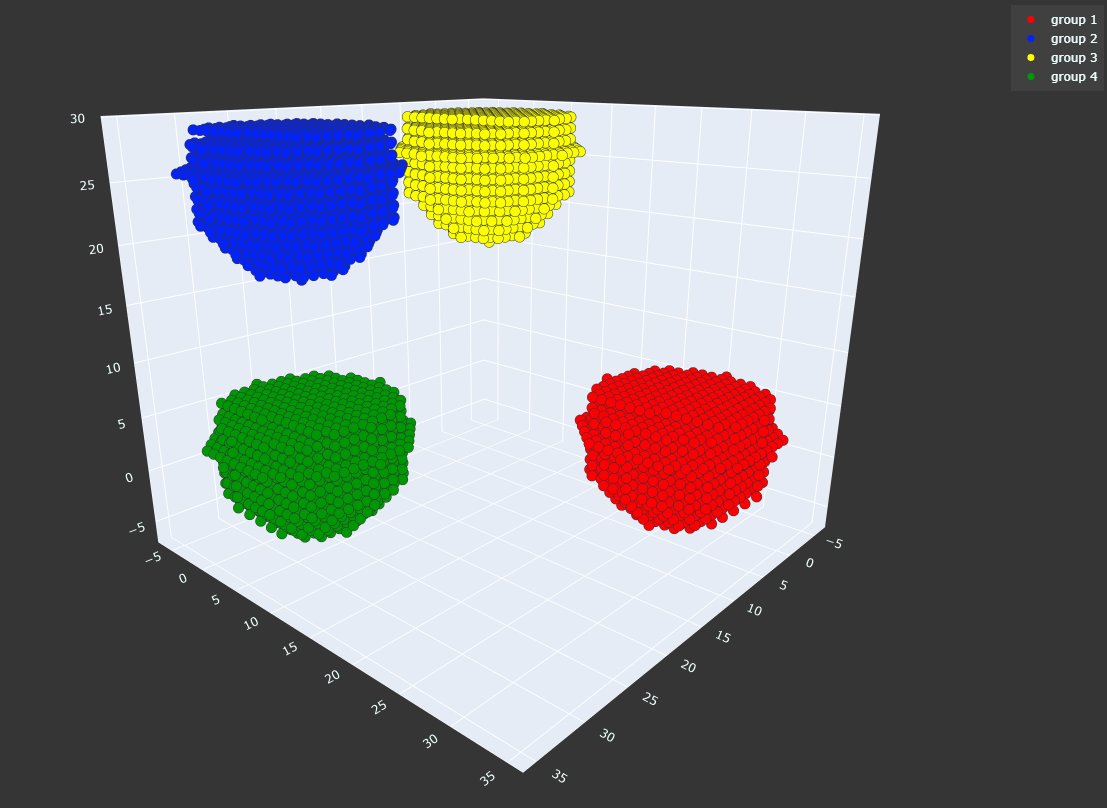
\includegraphics[width=0.75\linewidth]{images/groups.png}
    \caption{Network containing 4 groups with 2000 nodes per group}
    \label{fig:groups}
\end{figure}

To distribute the spheres in the coordinate system, it is first divided into cubes. Let $n_{max}$ be the number of nodes in the biggest group. To determine the side length $s$ of the cubes, it is necessary to know the radius $r$ of the smallest sphere that can fit $n_{max}$ nodes.

\subsection{Creating a sphere}
The nodes are placed only at coordinates $x,y,z \in \mathbb{N}$. To create a sphere that can fit $n_{max}$ nodes, the radius needs to be known before the exact coordinates are calculated. The problem with this is that the only way to get the exact radius for a sphere that can fit $n_{max}$ nodes that are all at coordinates $x,y,z \in \mathbb{N}$ is to use the algorithm depicted in \ref{alg:exact_radius}.
\begin{algorithm}
\caption{Calculating exact radius}
\label{alg:exact_radius}
\begin{algorithmic}
\Require {$(n_{max})$}
\Ensure {$r$}
\State $r \gets 0$
\State $n \gets 0$
\While{$n < n_{max}$}
    \State $r \gets r+1$
    \State coords $\gets$ calculate coordinates for all nodes in sphere with radius $r$
    \State $n \gets $ length of coords
\EndWhile
\end{algorithmic}
\end{algorithm}
This algorithm is inefficient because it computes all spheres until $r$ is big enough. This can be improved by estimating the number of nodes in a sphere of radius $r$ instead of computing the exact number. The number of nodes is estimated using the formula \ref{eq:sphere_lattice}.
\begin{equation}
\label{eq:sphere_lattice}
    \dfrac{4 \cdot \pi \cdot r^3}{3}
\end{equation}
This estimation incurs an error. \ref{eq:gauss_error} shows the best currently known formula for calculating this error which was discovered and proven by Zheng \cite{gaussSphereProblem}.
\begin{equation}
\label{eq:gauss_error}
    \sum_{\substack{x \in z^3 \\ |x| \leq r}}{P(x)} = O_{\epsilon, P}(r^{v + 84 / 63 + \epsilon})
\end{equation}
The true error bound is suspected to be $O_\epsilon(R^{1 + \epsilon})$ but this is currently not possible to prove. For the context of this work the simpler estimation shown in formula \ref{eq:gauss_error_rough} is sufficient.
\begin{equation}
\label{eq:gauss_error_rough}
    O_{\epsilon}(r^{21/16 + \epsilon})
\end{equation}

Let $r_e$ be the resulting radius required for $n_{max}$ nodes using the estimation. If $n_{max}$ is close to the boundary between two radii, then the resulting radius may be too large or too small due to the introduced error. For this reason, the resulting radius is decremented by one and the exact calculation is then used to find the correct required radius, as shown in algorithm \ref{alg:exact_radius_improved}. This will always find the smallest radius for a sphere containing at least $n_{max}$ points.

\begin{algorithm}
\caption{Calculating exact radius}
\label{alg:exact_radius_improved}
\begin{algorithmic}
\Require {$(n_{max})$}
\Ensure {$r$}
\State $r \gets 0$
\State $n \gets 0$
\While{$n < n_{max}$}
    \State $r \gets r + 1$
    \State $n \gets$ estimate amount of nodes in sphere with radius $r$
\EndWhile
\State $ r \gets r - 1$
\While{len(coords) $ < n_{max}$}
    \State coords $\gets$ calculate exact coords of nodes for radius $r$
\EndWhile
\end{algorithmic}
\end{algorithm}

The formula \ref{eq:sphere_inequality} represents the inequality for points inside or on the surface of a sphere centered at the origin in three-dimensional space, as proven by Gui and Moradifam \cite{sphereInequality}. A point is inside the sphere if this inequality is satisfied.
\begin{equation}
\label{eq:sphere_inequality}
    x^2 + y^2 + z^2 \leq r^2
\end{equation}
This means the bigger one of the values $x,y,z$ becomes, the smaller the other must be to satisfy the inequality. Using this knowledge, it is possible to construct an algorithm (shown in \ref{alg:calc_sphere_points}) that efficiently computes all triples of $x,y,z$ values that satisfy the inequality. The order of $z,x,y$ in the algorithm is important, so a half full sphere creates points that fill the sphere from the bottom to the top.
Starting with $z$ and $y=0$, transforming the formula to $x$ results in $|x| \leq \sqrt{(r^2 - z^2)}$, which corresponds to all possible values of $x$ with respect to $z$ and $r$. This range corresponds to $-a,a$ in the algorithm. Solving for $y$ then results in $|y| \leq \sqrt{(r^2 - z^2 - x^2)}$, which yields all possible values for $y$ with respect to $x,z,r$. This coincides with $-b,b$ in the algorithm.

\begin{algorithm}
\caption{Calculating lattice points}
\label{alg:calc_sphere_points}
\begin{algorithmic}
\Require {$r$}
\Ensure {$coords$}
\State $coords \gets []$
\For {$z := -r$ to $r$}
    \State $a \gets \lfloor\sqrt{(r^2 - z^2)}\rfloor$
    \For {$x := -a$ to $a$}
        \State $b \gets \lfloor\sqrt{(a^2 - x^2)}\rfloor$
        \For {$y := -b$ to $b$}
            \State coords $\gets (x,y,z)$
        \EndFor
    \EndFor
\EndFor
\end{algorithmic}
\end{algorithm}

The Python implementation of this function takes in an amount of points $n$ and returns a list of triples of length $n$ containing the resulting coordinates and the radius $r$ of the sphere.

\section{Arranging the spheres}
After calculating the coordinates and radii for each sphere (one for each group), the biggest radius $r_{max}$ is known. Using this, the side length of the cubes can be calculated. To create some space between the spheres, this side length $s$ is calculated as $s = 2 * r_{max} * 1.25$ to add an empty space of 12.5\% of the sphere diameter on each side.

The cubes are always created within a larger cube, e.g. the number of cubes is $c = x^3$. $x$ is the side length of the bigger cube in cubes (e.g. a side length of $x=3$ cubes results in $c=27$ smaller cubes). In order not to spread out the spheres unnecessarily, the smallest number of cubes should be created. The minimum required number of cubes is the number of spheres/groups. To get the next higher value for $c$, $x$ can be calculated by $x =\lceil\sqrt[3]{num\_groups}\rceil$.

Using this the algorithm \ref{alg:cube_offsets} computes the coordinates of bottom left corner of each cube.

\begin{algorithm}
\caption{Calculating cube offsets}
\label{alg:cube_offsets}
\begin{algorithmic}
\Require {$num\_group, r_{max}$}
\Ensure {$offsets$}
\State $s \gets \lceil 2 * r_{max} * 1.25\rceil$
\State $o \gets \lceil 2 * r_{max} * 0.125\rceil$
\State $c \gets \lceil\sqrt[3]{num\_groups}\rceil$
\For {$x,y,z := 0$ to $c$}
    \State offsets $\gets (x \cdot s + o, y \cdot s + o, z \cdot s + o)$
\EndFor
\end{algorithmic}
\end{algorithm}

For each sphere a random cube is selected and its offsets are added to the coordinates of all points within the sphere, resulting in the final coordinates for all nodes in the network.

\section{Creating the scatter graph}
\label{sub:scatter_graph}
In the final graph it must be possible to toggle the visibility of each group. To achieve this, the coordinates for each group are stored separately and only the active ones are added to the coordinate lists for the \texttt{Scatter3d} call.

\begin{lstlisting}[language=python, caption={Creation of the node trace}, label={lst:node_trace}]
for group in self.network.groups:
    if group.id not in self.hidden_groups:
        x, y, z = zip(*self.group_coords[group.id])
        aXn.extend(x)
        aYn.extend(y)
        aZn.extend(z)
        colors.extend([group.color] * len(x))
trace1 = go.Scatter3d(
    x=aXn,
    y=aYn,
    z=aZn,
    mode="markers",
    name="nodes",
    marker=dict(
        symbol="circle",
        size=6,
        color=colors,
        line=dict(color="rgb(50,50,50)", width=0.5),
    ),
    uirevision="0",
    showlegend=False,
)
\end{lstlisting}

The code in \ref{lst:node_trace} creates the trace that displays all active nodes. Whenever the visibility of a group is toggled, this trace must be rebuilt. It is important to note that the coordinates for the nodes in the x,y,z arrays contain the nodes in ascending order by their id. This means that nodes of group 0 come first starting with node 0, then group 1, and so on. This is important for creating color sequences based on the node states, which is discussed in section \ref{sec:color_sequence}.

\section{Displaying the edges}
The edges are displayed using a second \texttt{Scatter3d} with the \texttt{lines} mode. For this the x,y and z arrays need the format of [xStart, xEnd, None] for each line. This means that a coordinate array for 100 lines would have a length of 300.

The current format in which the edges are represented contains only the node ids that are connected by edges. This representation was created in section \ref{sub:havel_hakimi}. To translate these node ids to the coordinates of the nodes calculated in section \ref{sub:displayNodes}, a map is created when the coordinates are calculated for each node. This map stores the node id as a key and the index of its coordinates, in the coordinate array, as value. This map can be used to calculate the start and end coordinates for all edges of visible groups, which is done by looking up the coordinates of the start and end nodes by using their ids and the map. The python code that realizes this can be seen in listing \ref{lst:edge_creation}.
\begin{lstlisting}[language=python, caption={Creation of the edge coordinate arrays}, label={lst:edge_creation}]
 for edge in edges:
    _from, to = edge[0], edge[1]
    if not (_from in node_id_map and to in node_id_map):
        continue
    from_ind = node_id_map[_from]
    to_ind = node_id_map[to]
    aXe.extend([node_coords_x[from_ind], node_coords_x[to_ind], None])
    aYe.extend([node_coords_y[from_ind], node_coords_y[to_ind], None])
    aZe.extend([node_coords_z[from_ind], node_coords_z[to_ind], None])
\end{lstlisting}

The trace is then created using the \texttt{Scatter3d} call from listing \ref{lst:edge_trace}.
\begin{lstlisting}[language=python, caption={Creation of the edge trace}, label={lst:edge_trace}]
trace2 = go.Scatter3d(
            x=aXe,
            y=aYe,
            z=aZe,
            mode="lines",
            uirevision="0",
            line=dict(color="rgb(125,125,125)", width=1),
            hoverinfo="none",
            showlegend=False,
        )
    \end{lstlisting}